% 原书印刷28–31页，PDF物理59–62页；至§1.7前.
\subsection{密度函数与质量函数}\label{sec:1.6}
与随机变量$X$及其cdf $F_X$相关联的，还有另一个函数，称为概率密度函数（probability density function，pdf）或概率质量函数（probability mass function，pmf）.pdf与pmf分别对应连续和离散情形.它们都与随机变量的“点概率”有关.
\begin{definition}\label{def:1.6.1}\index{SI0850@概率质量函数}
离散随机变量$X$的概率质量函数（pmf）为
$$f_X(x)=P(X=x),\qquad\text{对所有$x$}.$$
\end{definition}

\begin{example}[几何分布的概率]\label{ex:1.6.2}\index{SI0321@概率质量函数}
对于例\ref{ex:1.5.4}中的几何分布，其pmf为
$$f_X(x)=P(X=x)=\begin{cases}(1-p)^{x-1}p,&x=1,2,\ldots,\\0,&\text{其他情形}.
\end{cases}$$
回忆一下，$P(X=x)$，等价地$f_X(x)$，就是cdf在$x$处的跳跃大小.我们可以用pmf计算概率.既然现在可以度量单个点的概率，只需对所考虑事件中的所有点求和即可.因此，对满足$a\le b$的正整数$a,b$，有
$$P(a\le X\le b)=\sum_{k=a}^b f_X(k)=\sum_{k=a}^b(1-p)^{k-1}p.$$
特别地，
\begin{equation}\label{eq:1.6.1}P(X\le b)=\sum_{k=1}^b f_X(k)=F_X(b).\end{equation}
\end{example}

我们采用一个广泛接受的约定：用大写字母表示cdf，用相应的小写字母表示pmf或pdf.

在连续情形下定义pdf时，需要稍加谨慎.若直接尝试计算连续随机变量的$P(X=x)$，会得到如下结果.由于对任意$\varepsilon>0$，有$\{X=x\}\subset\{x-\varepsilon<X\le x\}$，由定理\ref{thm:1.2.9}\hyperref[itm:thm:1.2.9:c]{(c)}得
$$P(X=x)\le P(x-\varepsilon<X\le x)=F_X(x)-F_X(x-\varepsilon),$$
对任意$\varepsilon>0$均成立.因此，由$F_X$的连续性，
$$0\le P(X=x)\le\lim_{\varepsilon\downarrow0}[F_X(x)-F_X(x-\varepsilon)]=0.$$
不过，只要理解pdf的用途，它的定义便会清楚.

由例\ref{ex:1.6.2}可见，pmf给出“点概率”.在离散情形中，对pmf的值求和就得到cdf（如\eqref{eq:1.6.1}）.连续情形中相应的做法，是以积分代替求和，得到
$$P(X\le x)=F_X(x)=\int_{-\infty}^x f_X(t)\,dt.$$
利用微积分基本定理，若$f_X(x)$连续，则进一步有
\begin{equation}\label{eq:1.6.2}\index{SI0448@微积分基本定理}\frac d{dx}F_X(x)=f_X(x).\end{equation}
注意，这与离散情形的类比几乎完全一致：将“点概率”$f_X(x)$“加起来”，便得到区间概率.

\sourcepageanchor{60}

\begin{definition}\label{def:1.6.3}\index{SI0828@概率密度函数}
连续随机变量$X$的概率密度函数（pdf）$f_X(x)$是满足下式的函数：
\begin{equation}\label{eq:1.6.3}F_X(x)=\int_{-\infty}^x f_X(t)\,dt,\qquad\text{对所有$x$}.\end{equation}
\end{definition}

\emph{记号说明：}“$X$的分布由$F_X(x)$给出”可简记为“$X\sim F_X(x)$”，其中符号“$\sim$”读作“服从”.类似地，可写$X\sim f_X(x)$；若$X$与$Y$同分布，也可写$X\sim Y$.

在连续情形中，描述区间概率时可以略微随意一些.因为连续随机变量满足$P(X=x)=0$，所以
$$P(a<X<b)=P(a<X\le b)=P(a\le X<b)=P(a\le X\le b).$$
应当清楚，pdf（或pmf）包含的信息与cdf相同.因此，解题时可以使用其中任何一个，并应尽量选择较简单的那个.


\sourcepageanchor{61}

\begin{figure}[htbp]\centering
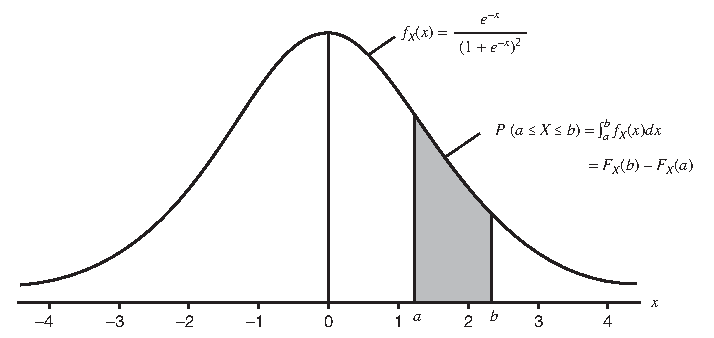
\includegraphics[width=.88\textwidth]{assets/chapter1/fig-1-6-1.pdf}
\caption{Logistic曲线下的面积}\label{fig:1.6.1}
\end{figure}
\FloatBarrier
\begin{example}[Logistic分布的概率]\label{ex:1.6.4}\index{SI0331@概率密度函数}
对于例\ref{ex:1.5.5}中的Logistic分布，有
$$F_X(x)=\frac1{1+e^{-x}},$$
因此
$$f_X(x)=\frac d{dx}F_X(x)=\frac{e^{-x}}{(1+e^{-x})^2}.$$
曲线$f_X(x)$下的面积给出区间概率（见图\ref{fig:1.6.1}）：
\begin{equation*}\begin{aligned}
P(a<X<b)&=F_X(b)-F_X(a)\\
&=\int_{-\infty}^b f_X(x)\,dx-\int_{-\infty}^a f_X(x)\,dx\\
&=\int_a^b f_X(x)\,dx.
\end{aligned}\end{equation*}
\end{example}

对于pdf（或pmf），实际上只有两个要求，它们都是定义的直接结果.
\begin{theorem}\label{thm:1.6.5}\index{SI0838@性质}\index{SI0856@性质}
函数$f_X(x)$是某个随机变量$X$的pdf（或pmf），当且仅当
\begin{enumerate}[label=\alph*.]
\item 对所有$x$都有$f_X(x)\ge0$.
\item $\sum_x f_X(x)=1$（pmf），或$\int_{-\infty}^{\infty}f_X(x)\,dx=1$（pdf）.
\end{enumerate}
\end{theorem}
\begin{proof}
若$f_X(x)$是pdf（或pmf），两个性质由定义立即得到.特别地，对pdf，利用\eqref{eq:1.6.3}和定理\ref{thm:1.5.3}，有
$$1=\lim_{x\to\infty}F_X(x)=\int_{-\infty}^{\infty}f_X(t)\,dt.$$
反向蕴含同样容易证明.\index{SI0831@构造}\semanticindexanchor{831:61}\index{SI0852@构造}\semanticindexanchor{852:61}一旦有了$f_X(x)$，就可以定义$F_X(x)$，并应用定理\ref{thm:1.5.3}.
\end{proof}


\sourcepageanchor{62}

从纯数学的观点看，任何具有有限正积分（或和）的非负函数，都能转化为pdf或pmf.例如，若$h(x)$为任意非负函数，在集合$A$上为正，其他地方为0，且对某个常数$K>0$有
$$\int_{\{x\in A\}}h(x)\,dx=K<\infty,$$
则$f_X(x)=h(x)/K$是某个取值于$A$的随机变量$X$的pdf.

事实上，关系\eqref{eq:1.6.3}并非总成立，因为$F_X(x)$可能连续却不可微.确实存在这样的连续随机变量：无论选择什么$f_X(x)$，该积分关系都不成立.这些情形相当病态，我们将忽略它们.因此，本书假设每个连续随机变量都满足\eqref{eq:1.6.3}.在更高等的教材中（例如\hyperref[bib:source33]{Billingsley，1995，第31节}），若随机变量满足\eqref{eq:1.6.3}，则称其为绝对连续（absolutely continuous）.\index{SI0865@绝对连续}\semanticindexanchor{865:62}
